\chapter{Risultati sperimentali}
Per valutare le performance delle funzioni sviluppate, sono stati eseguiti 10 cicli incrementali per ciascuna funzionalità sviluppata, eccezion fatta per il docking la cui esecuzione con tutti i dati di input (289 ligandi, 11 recettori) presi in esame ha richiesto circa 3 giorni di esecuzione.\newline
Tutti i test sono stati eseguiti su \href{https://colab.research.google.com/}{Google Colaboratory} (Colab). Colab è una piattaforma gratuita che permette a chiunque di scrivere ed eseguire codice Python attraverso un browser. L’unico requisito è possedere un account Google (ad esempio Gmail). Colab è basato su un progetto Open Source chiamato \href{https://jupyter.org/}{Jupyter}. I documenti/programmi scritti su Colab sono chiamati Notebook e verranno salvati automaticamente sul Google Drive associato al proprio account.\newline
Le macchine virtuali messe a disposizione in Google Colab ospitano un ambiente configurato che consente di concentrarsi sin da subito sui progetti di Data Science:  sono presenti numerose librerie Python, tra cui moltissime di Data Science, si può usufruire di GPU e TPU per dare boost computazionali importanti ai lavori.\newline
Per facilitare la comprensione dei risultati ottenuti sono stati realizzati dei grafici, uno per ciascuna funzionalità testata.\newline
Ogni grafico riporta l'andamento dei tempi in funzione dell'incremento degli input relativi.\newline
Di seguito sono riportati i grafici relativi ai test effettuati per le funzioni:
\begin{itemize}
    \item Preparazione dei ligandi
    \item Preparazione dei recettori
    \item Esecuzione dell'analisi.
\end{itemize}

\begin{figure}[H]
    \centering
    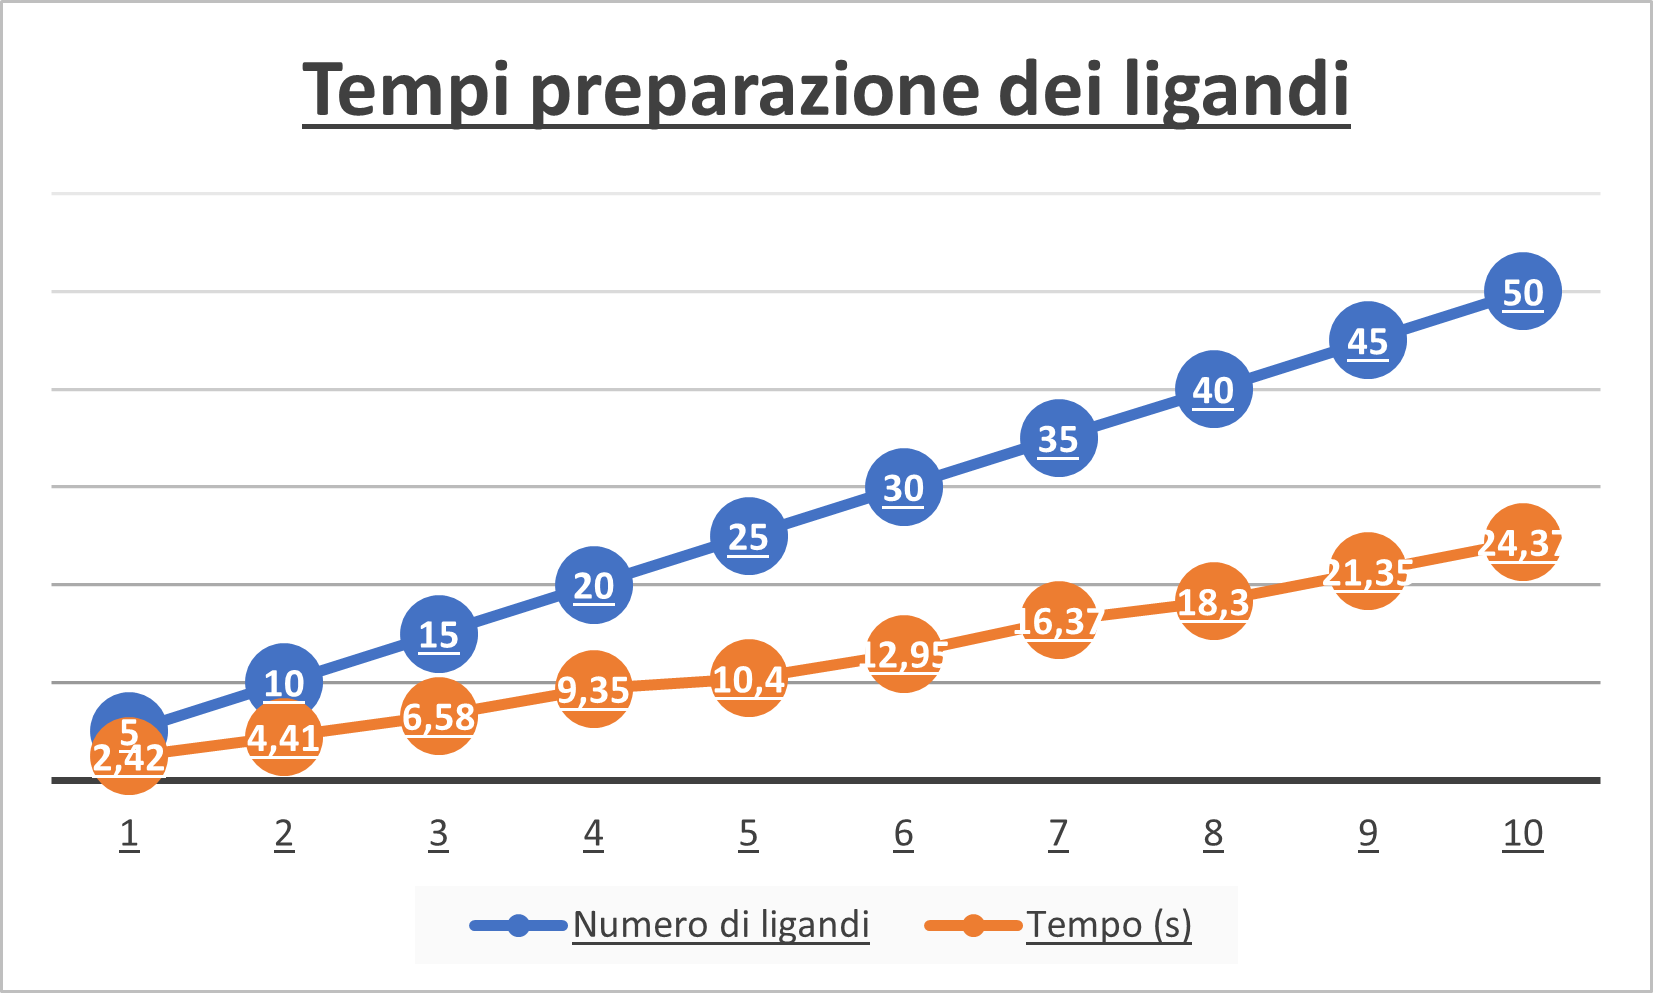
\includegraphics{immagini/capitolo4/tempiLigandi.png}
    \caption{Tempi di preparazione dei ligandi}
    \label{fig:tempi ligandi}
\end{figure}

\begin{figure}[H]
    \centering
    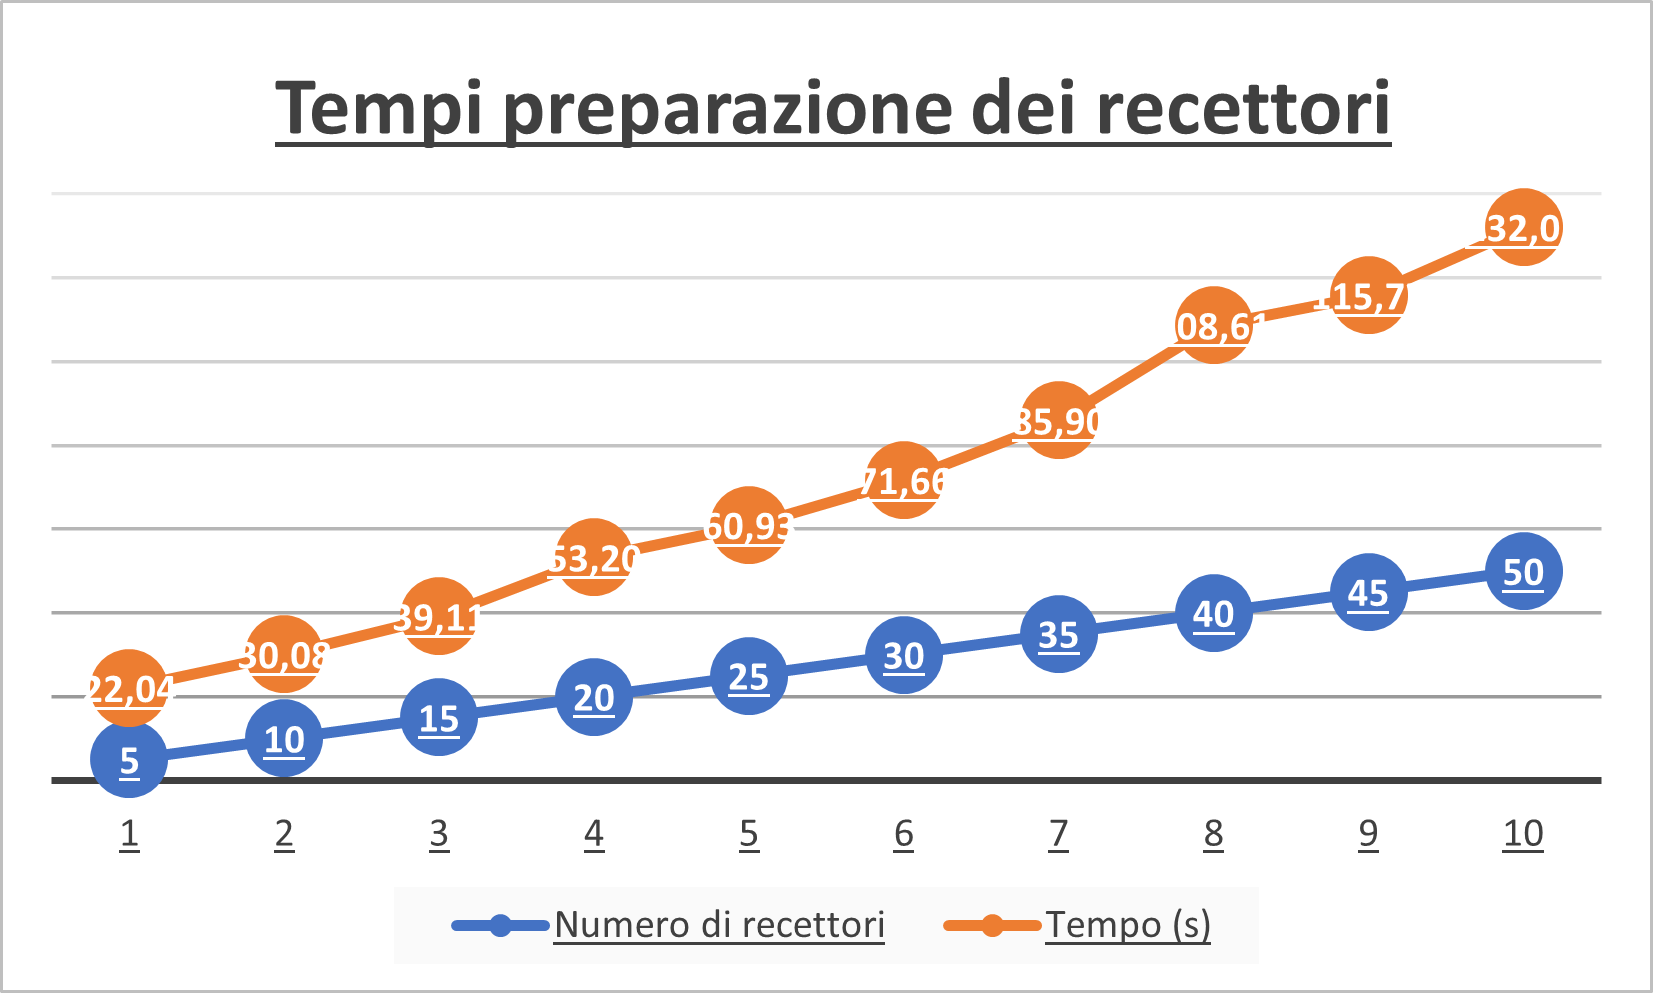
\includegraphics{immagini/capitolo4/tempiRecettori.png}
    \caption{Tempi di preparazione dei recettori}
    \label{fig:tempi recettori}
\end{figure}

\begin{figure}[H]
    \centering
    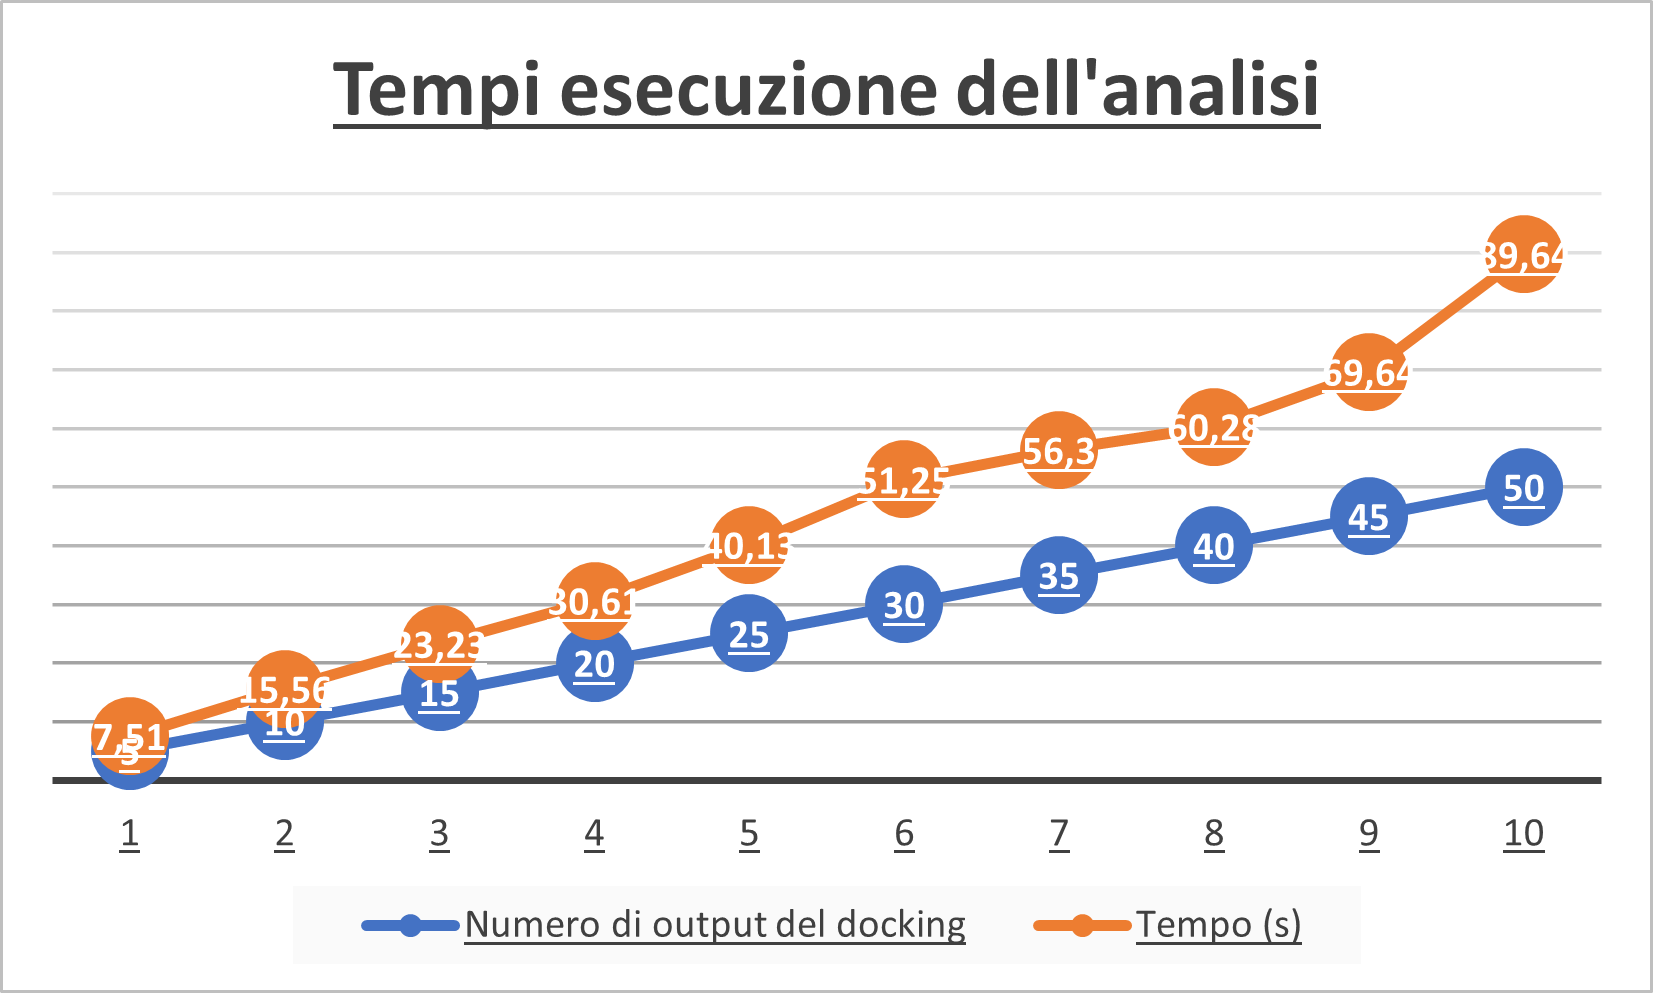
\includegraphics{immagini/capitolo4/tempiAnalisi.png}
    \caption{Tempi di esecuzione dell'analisi}
    \label{fig:tempi analisi}
\end{figure}

Osservando e comparando i dati dei grafici sopra, si può notare che:

\begin{itemize}
    \item le prestazioni delle funzioni, preparazione ligandi, preparazione recettori e analisi rispecchiano la stessa complessità di tempo
    \item le prestazioni del sistema in generale non degradano con il crescere dei dati in input
    \item l'andamento dei tempi si incrementa linearmente con l'aumentare dell'input.
\end{itemize}